\documentclass{beamer}
\usepackage{tcolorbox}

%\beamerdefaultoverlayspecification{<+->}
\newcommand{\data}{\mathcal{D}}

\DeclareMathOperator*{\argmax}{arg\,max}

\newcommand\Item[1][]{%
	\ifx\relax#1\relax  \item \else \item[#1] \fi
	\abovedisplayskip=0pt\abovedisplayshortskip=0pt~\vspace*{-\baselineskip}}
\usepackage{amsmath}
\usepackage{amssymb}


\usetheme{metropolis}           % Use metropolis theme


\title{Bayesian Machine Learning, MLE, MAP - II}
\date{\today}
\author{Nipun Batra}
\institute{IIT Gandhinagar}
\begin{document}

\maketitle
\begin{frame}{Fully Bayesian Approach}
\begin{itemize}
\item MLE and MAP do not give us uncertainty.
\begin{figure}[htp]
    \centering
    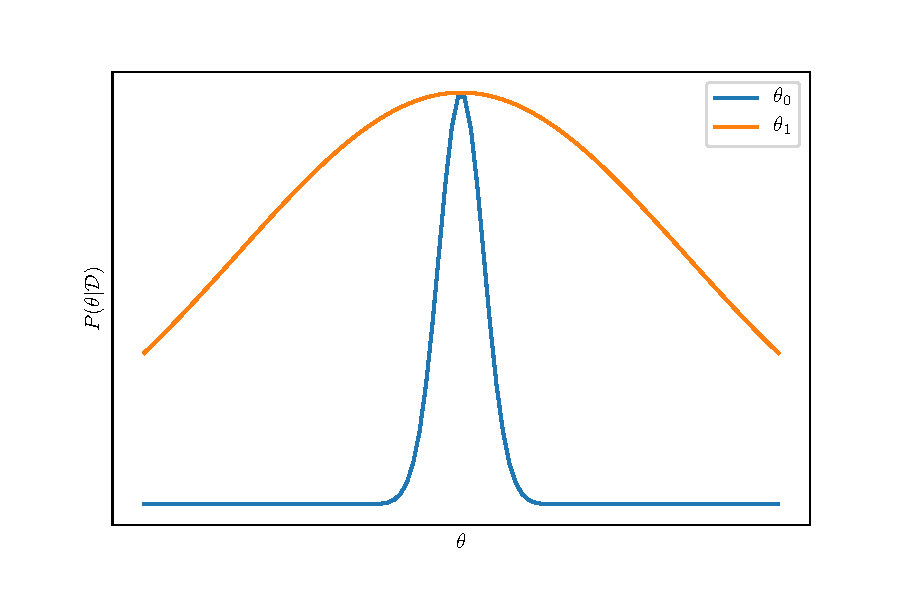
\includegraphics[width=6cm]{plots/fullybayesian1.pdf}
    \caption{More uncertainty around $\theta_0$ than $\theta_1$}
    \label{fig:online}
\end{figure}
\end{itemize}
\end{frame}


\begin{frame}{Predictive Distribution for the Coin Toss Problem}
\begin{itemize}
\item $P(\text{Next Toss} = H | \text{ Data})$
\item What value of $\theta$ should be used?
\item Answer: Use all the possible values of $\theta$.
\item  $P(\text{Next Toss} = H | Data)$ = $\int P(\text{Next Toss} = H, \theta | \text{ Data})d\theta$ Why?
\item  Marginalization! $p(x) = \int_y p(x,y)dy$
\item Note that the conditioning above is only over the observed data or evidence.
\end{itemize}
\end{frame}
\begin{frame}{Predictive Distribution for the Coin Toss Problem if $\theta$ is known}

\begin{itemize}
	
	\item Let $c$ be a random variable that is assigned the value $1$ if head results after tossing a coin and 0 if tail results after tossing a coin.
	\item  Question: What is $P(\text{Next Toss} = c | \theta)$?
	\item Answer: $\theta^c(1 - \theta)^{1-c}$. Why?
	\item Suppose c = 0. Then $P(\text{Tails} | \theta)$ = $(1 - \theta)$.
\end{itemize}
\end{frame}

\begin{frame}{Predictive Distribution for the Coin Toss Problem}

\begin{itemize}
	
	\item Let us consider the case where we have a Beta prior for our coin toss problem. What is the predictive distribution, given we have observed some data?
	\item Answer: $P(\text{Next} = c | \mathcal{D}, a, b )$ = $\int P(\text{Next =}c, \theta | \mathcal{D}, a, b)d\theta$
	\item From the chain rule of probability, we have the following:
	\begin{align*}
	    P(AB|CDE) = \frac{P(ABCDE)}{P(CDE)} = \frac{P(A|BCDE)P(BCDE)}{P(CDE)}
	\end{align*}
	\begin{align*}
	    = P(A|BCDE)P(B|CDE)
	\end{align*}
	
	
\end{itemize}
\end{frame}

\begin{frame}{Predictive Distribution for the Coin Toss Problem}

\begin{itemize}
	
	\item In our case, the integrand $P(\text{Next =}c, \theta |  \mathcal{D}, a, b)$ therefore becomes, $ P(\text{Next =}c, | \theta,  \mathcal{D}, a, b)P(\theta|\mathcal{D}, a, b)$
	\item If $\theta$ is known, then $P(\text{Next =}c | \theta,  \mathcal{D}, a, b) = P(\text{Next =}c | \theta)$. Why? 
	\item This is because we know the actual model parameter distribution. The data \emph{cannot} affect it. What about a and b affecting the prior? They do not concern us anymore either, since we actually know the parameters. 
	\item $\implies$ The predictive distribution is, 
	\begin{align*}
	    \int_\theta \theta^c(1 - \theta)^{1-c}\frac{\Gamma(n_H + n_T + a + b)\theta^{n_H + a - 1}(1 - \theta)^{n_T + b - 1}d\theta}{\Gamma(n_H + a)\Gamma(n_T + b)}
	\end{align*}
	
	
\end{itemize}
\end{frame}
\begin{frame}{Predictive Distribution for the Coin Toss Problem}
\begin{align*}
     = \frac{\Gamma(n_H + n_T + a + b)}{\Gamma(n_H + a)\Gamma(n_T + b)}\int_\theta \theta^{n+h + a - 1 + c}(1 - \theta)^{n_T + b - c}d\theta
\end{align*}
\begin{align*}
   =   \frac{\Gamma(n_H + n_T + a + B)\Gamma(c + n_H + a)\Gamma(n_T + b - c + 1)}{\Gamma(n_H + a)\Gamma(n_T + b)\Gamma(1 + n_H + a + n_T + b)}
\end{align*}
    
\end{frame}


\end{document}
